\documentclass{ximera}

% MATH -----------------------------------------------------------
\newcommand{\nats}{\mathbb N}
\newcommand{\ints}{\mathbb Z}
\newcommand{\rats}{\mathbb Q}
\newcommand{\reals}{\mathbb R}
\newcommand{\complex}{\mathbb C}
\newcommand{\powerset}{\mathscr P}

%-------------------------------------------------------------

\pgfplotsset{compat=1.18}
\begin{document}
\begin{abstract}
 \end{abstract}

    \title{Exemplar Examples 1}
    
    \maketitle

Let's consider the first order linear differential equation $y^{\,\prime}=2x\left(e^{-x^2}-2y\right)$.

\begin{enumerate}

\item Here is an (approximate) direction field for this differential equation on \\$[-2,2]\times [-2,2]$.  Let's draw (part of) the solution curve to this differential equation that passes through the point $(0,1)$.  Let's use our drawing to estimate the value of this solution when $x=1$.


\begin{figure}[h]
\centering
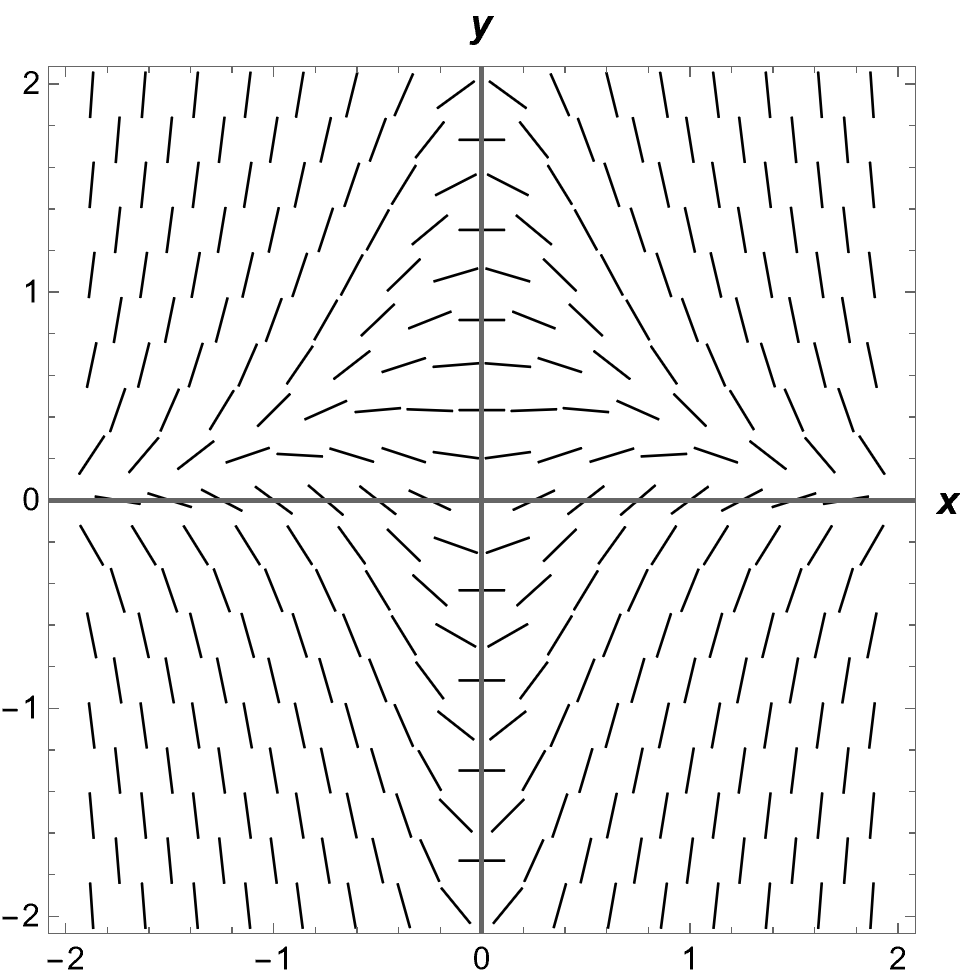
\includegraphics[scale=0.65,alt={A direction field.}]{ExemplarOneDirectionField.png}
   \caption{A direction field}
\end{figure}


\item Let's write this equation in standard form.

\vfill


\item Let's determine an integrating factor.

\vfill

\newpage 


\item Now let's solve this differential equation for its general solution, and determine the solution that passes through $(0,1)$.

\vfill

\vfill

\item  How good was our estimate?

\vfill


\end{enumerate}


\end{document}